% Regenerate with latex and dvisvgm; see graph-matching-common.tex.
% Shared styles for the vector replacements in graph-matching/.
% Compile each diagram from this directory, for example:
% latex -interaction=nonstopmode -halt-on-error augment-1.tex
% dvisvgm --no-fonts --exact --bbox=papersize -o augment-1.svg augment-1.dvi
\documentclass[tikz,border=5pt]{standalone}
\usepackage{lmodern,amssymb}
\usetikzlibrary{arrows.meta,backgrounds,calc}
\definecolor{matchred}{HTML}{D7191C}
\definecolor{matchblue}{HTML}{1748B5}
\definecolor{blossomgreen}{HTML}{087A16}
\definecolor{blossomfill}{HTML}{B3E3AF}
\tikzset{
  diagram/.style={x=1mm,y=-1mm,font=\small,line width=.6pt,
    line cap=round,line join=round,
    background rectangle/.style={fill=white},show background rectangle},
  vertex/.style={circle,draw,fill=white,minimum size=5mm,inner sep=0pt},
  point/.style={circle,fill=black,minimum size=2.8mm,inner sep=0pt},
  exposed/.style={point,draw=matchred,fill=matchred!80,line width=1pt},
  matching/.style={line width=2pt},
  transition/.style={-{Stealth[length=4mm,width=3mm]},
    line width=1.4pt,draw=matchblue},
  blossom/.style={draw=blossomgreen,fill=blossomfill,line width=1pt},
  route/.style={draw=matchred,line width=.9pt},
  label/.style={inner sep=1.5pt,align=center},
}

% The five-cycle has exactly two matching edges. Its exposed base is b0.
% Call inside a scope to translate the entire blossom consistently.
\newcommand{\FiveBlossom}{%
  \draw[blossom] (16,0) circle[radius=22mm];
  \foreach \id/\px/\py in {b0/0/0,b1/12/-16,b2/29/-9,b3/29/10,b4/11/16}
    \node[point] (\id) at (\px,\py) {};
  \draw (b0) -- (b1) (b2) -- (b3) (b4) -- (b0);
  \draw[matching] (b1) -- (b2) (b3) -- (b4);
  \node[label,text=blossomgreen,above] at (16,-22) {blossom};
  \node[label,text=blossomgreen,above=.3mm,xshift=-2mm] at (b0.north) {root};
  \node[label,below=.5mm] at (b0.south) {$v$};
}

\tikzset{
  operation vertex/.style={vertex,minimum size=4mm,font=\small},
  % Keep the white gap visible at the SVG's normal display size, both
  % along matched edges and around even roots and contracted blossoms.
  double stroke/.style={double=white,double distance=1.6pt,line width=.45pt},
  tree root/.style={operation vertex,double stroke},
  matched edge/.style={double stroke},
  new edge/.style={dashed,line width=.7pt},
  operation arrow/.style={-{Stealth[length=3.5mm,width=3mm]},
    line width=1.7pt,black!60},
}
\begin{document}
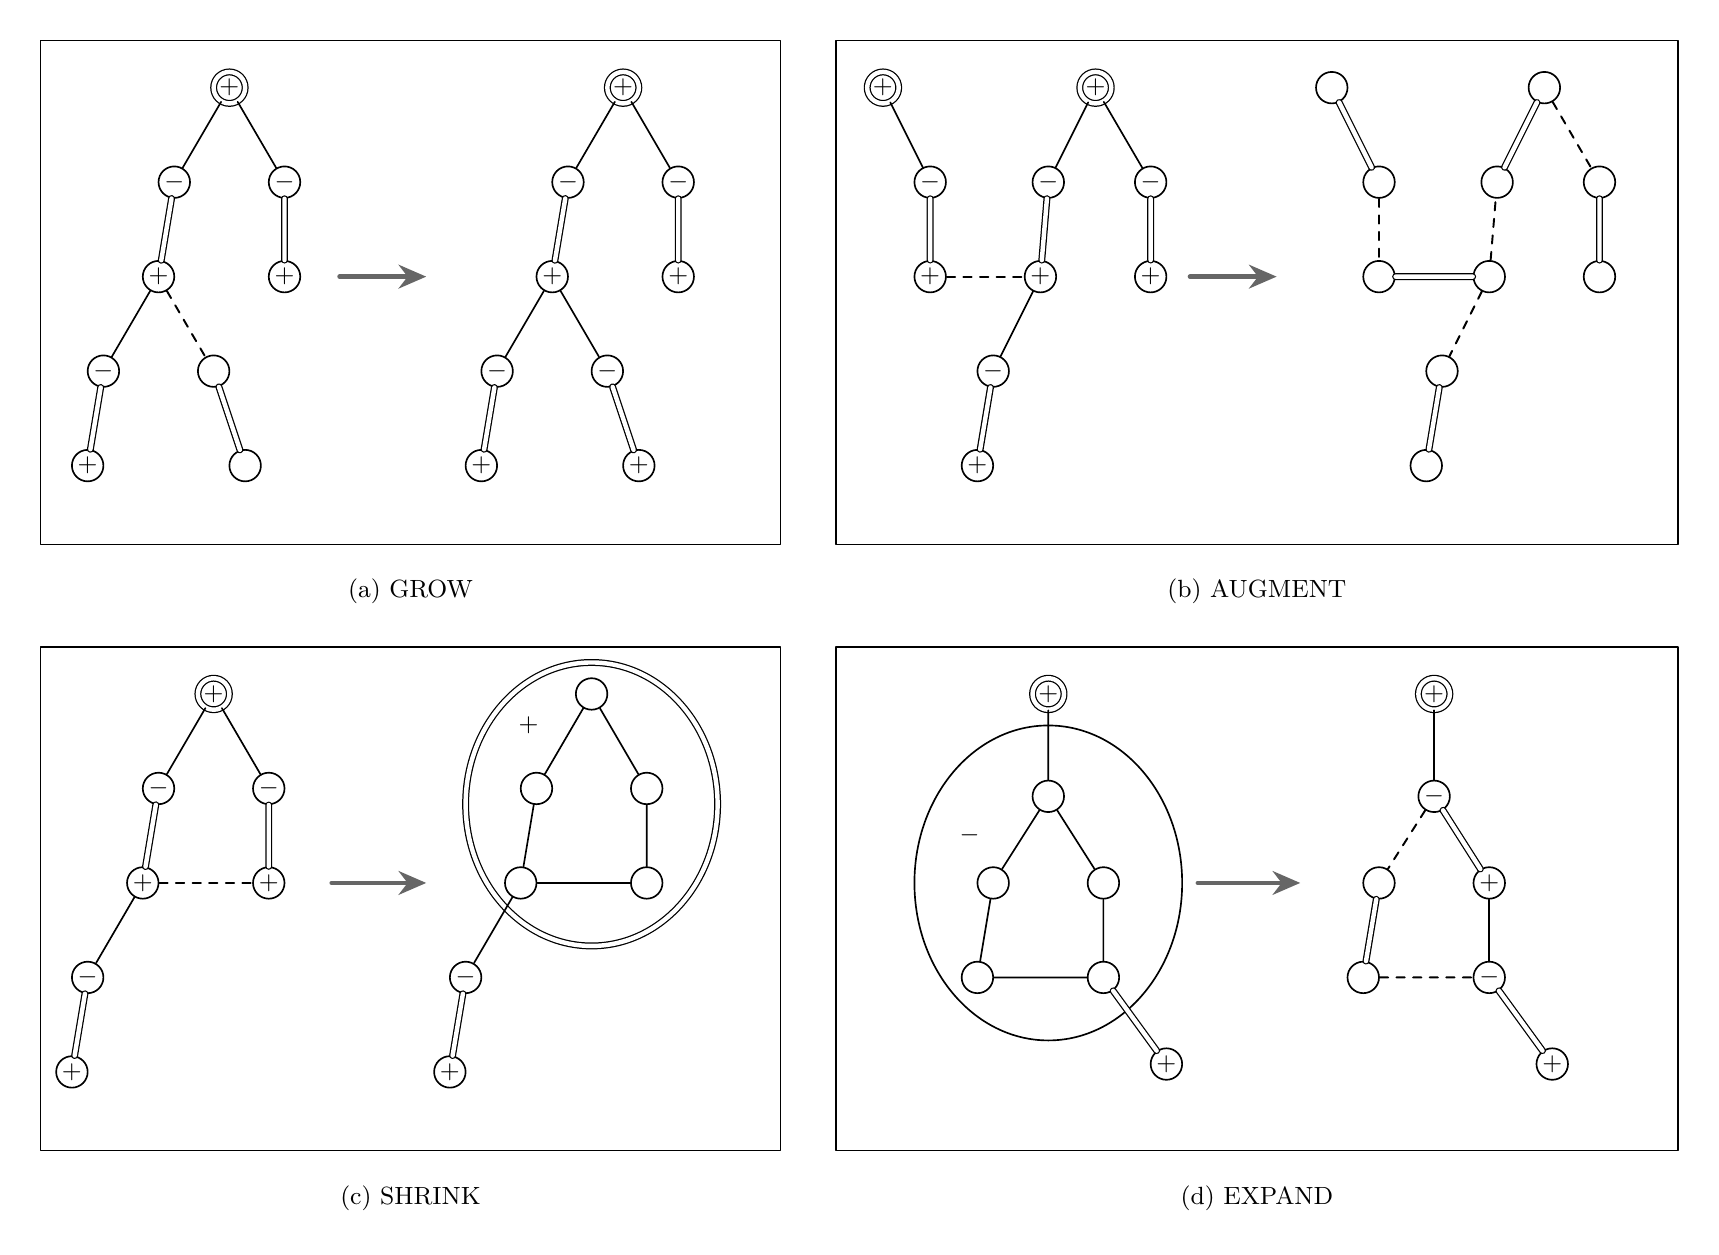
\begin{tikzpicture}[diagram]
  \draw (0,0) rectangle (94,64) (101,0) rectangle (208,64)
    (0,77) rectangle (94,141) (101,77) rectangle (208,141);
  \node[label] at (47,70) {(a) GROW};
  \node[label] at (154.5,70) {(b) AUGMENT};
  \node[label] at (47,147) {(c) SHRINK};
  \node[label] at (154.5,147) {(d) EXPAND};

  % GROW: the dashed edge reaches an unvisited matched pair. It becomes
  % a tree edge, and the pair receives odd/even labels (-/+).
  \foreach \state/\offset in {0/0,1/50} {
    \begin{scope}[xshift=\offset mm]
      \node[tree root] (r) at (24,6) {$+$};
      \node[operation vertex] (a) at (17,18) {$-$};
      \node[operation vertex] (b) at (31,18) {$-$};
      \node[operation vertex] (c) at (15,30) {$+$};
      \node[operation vertex] (d) at (31,30) {$+$};
      \node[operation vertex] (e) at (8,42) {$-$};
      \node[operation vertex] (f) at (6,54) {$+$};
      \ifnum\state=0
        \node[operation vertex] (g) at (22,42) {};
        \node[operation vertex] (h) at (26,54) {};
        \draw[new edge] (c) -- (g);
      \else
        \node[operation vertex] (g) at (22,42) {$-$};
        \node[operation vertex] (h) at (26,54) {$+$};
        \draw (c) -- (g);
      \fi
      \draw (r) -- (a) (r) -- (b) (c) -- (e);
      \draw[matched edge] (a) -- (c) (b) -- (d) (e) -- (f) (g) -- (h);
    \end{scope}
  }
  \draw[operation arrow] (38,30) -- (49,30);

  % AUGMENT: connect even vertices from distinct trees and flip the path
  % between their roots. The two off-path matched edges are retained.
  \begin{scope}[xshift=101mm]
    \foreach \state/\offset in {0/0,1/57} {
      \begin{scope}[xshift=\offset mm]
        \ifnum\state=0
          \node[tree root] (lr) at (6,6) {$+$};
          \node[tree root] (rr) at (33,6) {$+$};
          \foreach \id/\px/\py/\parity in {a/12/18/-,c/12/30/+,b/27/18/-,
              d/26/30/+,g/20/42/-,h/18/54/+,f/40/18/-,e/40/30/+}
            \node[operation vertex] (\id) at (\px,\py) {$\parity$};
          \draw (lr) -- (a) (rr) -- (b) (rr) -- (f) (d) -- (g);
          \draw[matched edge] (a) -- (c) (b) -- (d) (f) -- (e) (g) -- (h);
          \draw[new edge] (c) -- (d);
        \else
          \foreach \id/\px/\py in {lr/6/6,rr/33/6,a/12/18,c/12/30,b/27/18,
              d/26/30,g/20/42,h/18/54,f/40/18,e/40/30}
            \node[operation vertex] (\id) at (\px,\py) {};
          \draw[matched edge] (lr) -- (a) (c) -- (d) (b) -- (rr)
            (f) -- (e) (g) -- (h);
          \draw[new edge] (a) -- (c) (d) -- (b) (rr) -- (f) (d) -- (g);
        \fi
      \end{scope}
    }
    \draw[operation arrow] (45,30) -- (56,30);
  \end{scope}

  % SHRINK: a new edge closes a five-cycle at an even root. Contract it
  % to a single even blossom; the external branch remains alternating.
  \begin{scope}[shift={(0,77)}]
    \node[tree root] (r) at (22,6) {$+$};
    \foreach \id/\px/\py/\parity in {a/15/18/-,b/29/18/-,c/13/30/+,
        d/29/30/+,e/6/42/-,f/4/54/+}
      \node[operation vertex] (\id) at (\px,\py) {$\parity$};
    \draw (r) -- (a) (r) -- (b) (c) -- (e);
    \draw[matched edge] (a) -- (c) (b) -- (d) (e) -- (f);
    \draw[new edge] (c) -- (d);
    \draw[double stroke] (70,20) ellipse[x radius=16mm,y radius=18mm];
    \foreach \id/\px/\py in {r/70/6,a/63/18,b/77/18,c/61/30,d/77/30}
      \node[operation vertex] (\id) at (\px,\py) {};
    \node[operation vertex] (e) at (54,42) {$-$};
    \node[operation vertex] (f) at (52,54) {$+$};
    \draw (r) -- (a) -- (c) -- (d) -- (b) -- (r) (c) -- (e);
    \draw[matched edge] (e) -- (f);
    \node[label] at (62,10) {$+$};
    \draw[operation arrow] (37,30) -- (49,30);
  \end{scope}

  % EXPAND: retain the alternating path through an odd blossom. The
  % other matched pair is no longer part of the alternating tree.
  \begin{scope}[shift={(101,77)}]
    \draw (27,30) ellipse[x radius=17mm,y radius=20mm];
    \node[tree root] (r) at (27,6) {$+$};
    \foreach \id/\px/\py in {a/27/19,b/20/30,c/34/30,d/18/42,e/34/42}
      \node[operation vertex] (\id) at (\px,\py) {};
    \node[operation vertex] (f) at (42,53) {$+$};
    \draw (r) -- (a) -- (b) -- (d) -- (e) -- (c) -- (a);
    \draw[matched edge] (e) -- (f);
    \node[label] at (17,24) {$-$};
    \node[tree root] (r) at (76,6) {$+$};
    \node[operation vertex] (a) at (76,19) {$-$};
    \node[operation vertex] (b) at (69,30) {};
    \node[operation vertex] (c) at (83,30) {$+$};
    \node[operation vertex] (d) at (67,42) {};
    \node[operation vertex] (e) at (83,42) {$-$};
    \node[operation vertex] (f) at (91,53) {$+$};
    \draw (r) -- (a) (c) -- (e);
    \draw[matched edge] (a) -- (c) (b) -- (d) (e) -- (f);
    \draw[new edge] (a) -- (b) (d) -- (e);
    \draw[operation arrow] (46,30) -- (59,30);
  \end{scope}
\end{tikzpicture}
\end{document}
